\documentclass[tikz,border=3pt]{standalone}
\usepackage[T1]{fontenc}
\usepackage{lmodern,pgfplots}
\pgfplotsset{compat=1.18}
\definecolor{gapblue}{HTML}{4477AA}
\definecolor{directgreen}{HTML}{228833}
\definecolor{inkgray}{HTML}{343A40}
\definecolor{gridgray}{HTML}{DEE3E8}
\begin{document}
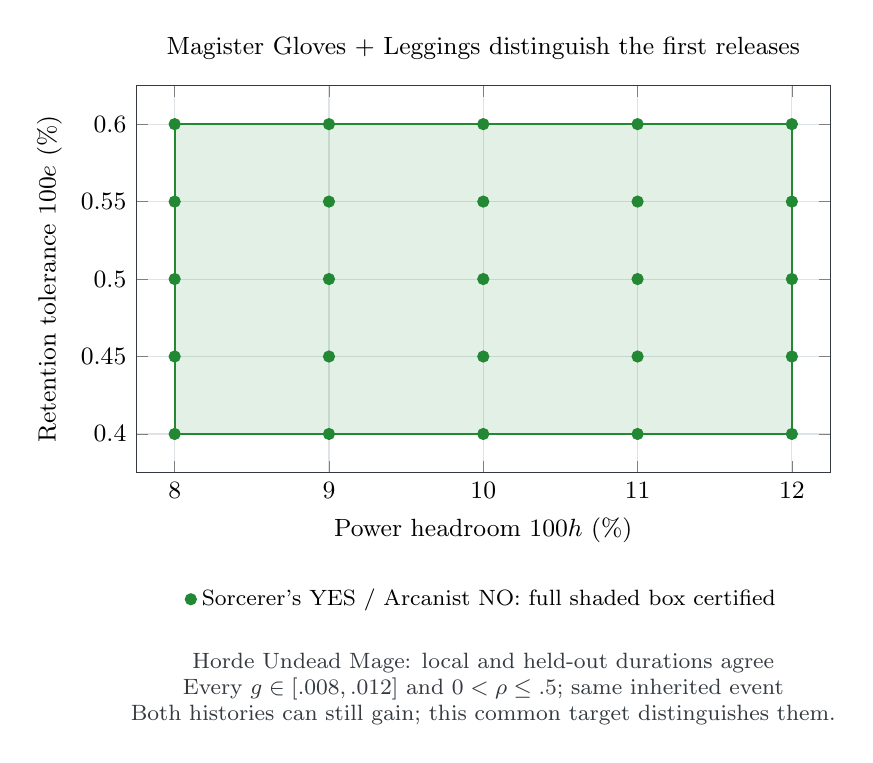
\begin{tikzpicture}
\begin{axis}[width=10.4cm,height=6.5cm,font=\small,clip=false,
 title={Magister Gloves + Leggings distinguish the first releases},
 title style={font=\small,align=center},
 xlabel={Power headroom $100h$ (\%)},ylabel={Retention tolerance $100e$ (\%)},
 xmin=7.75,xmax=12.25,ymin=.375,ymax=.625,
 xtick={8,9,10,11,12},ytick={.4,.45,.5,.55,.6},
 grid=both,grid style={gridgray},axis line style={inkgray},
 legend style={at={(.5,-.27)},anchor=north,draw=none,font=\footnotesize,legend columns=1}]
\fill[directgreen,opacity=.13] (axis cs:8,.4) rectangle (axis cs:12,.6);
\draw[directgreen,thick] (axis cs:8,.4) rectangle (axis cs:12,.6);
\addplot[only marks,mark=*,directgreen] coordinates {
 (8,.4)(8,.45)(8,.5)(8,.55)(8,.6)
 (9,.4)(9,.45)(9,.5)(9,.55)(9,.6)
 (10,.4)(10,.45)(10,.5)(10,.55)(10,.6)
 (11,.4)(11,.45)(11,.5)(11,.55)(11,.6)
 (12,.4)(12,.45)(12,.5)(12,.55)(12,.6)};
\addlegendentry{Sorcerer's YES / Arcanist NO: full shaded box certified}
\node[anchor=north,align=center,font=\footnotesize,text=inkgray] at (axis description cs:.5,-.44)
 {Horde Undead Mage: local and held-out durations agree\\
  Every $g\in[.008,.012]$ and $0<\rho\le.5$; same inherited event\\
  Both histories can still gain; this common target distinguishes them.};
\end{axis}
\end{tikzpicture}
\end{document}
